%# -*- coding: utf-8-unix -*-
% !TEX program = xelatex
% !TEX root = ../thesis.tex

\chapter{Data Processing}

\todo{chapter introduction}

\section{Data Overview}

    ACM Honors Class\cite{acmclass} of Shanghai Jiao Tong University is a elite program
    that cultivates computer scientists and top tier leaders.
    It has won the champion of ACM-ICPC for several times.
    And many students in ACM Honors Class have OI backgrounds.
    \todo{rephrase}

    The Online Judge\cite{acmoj} of ACM Honors Class starts in late 2011.
    At first, it only served the internal needs of ACM Honors Class.
    Programming-related courses such as C++ Programming, Data Structures,
    and Principle and Practice of Computer Algorithms,
    used the Online Judge to assign homework and hold exams.
    The ACM-ICPC team of SJTU organized several selection contests on the online judge.

    \begin{figure}[htp]
        \centering
        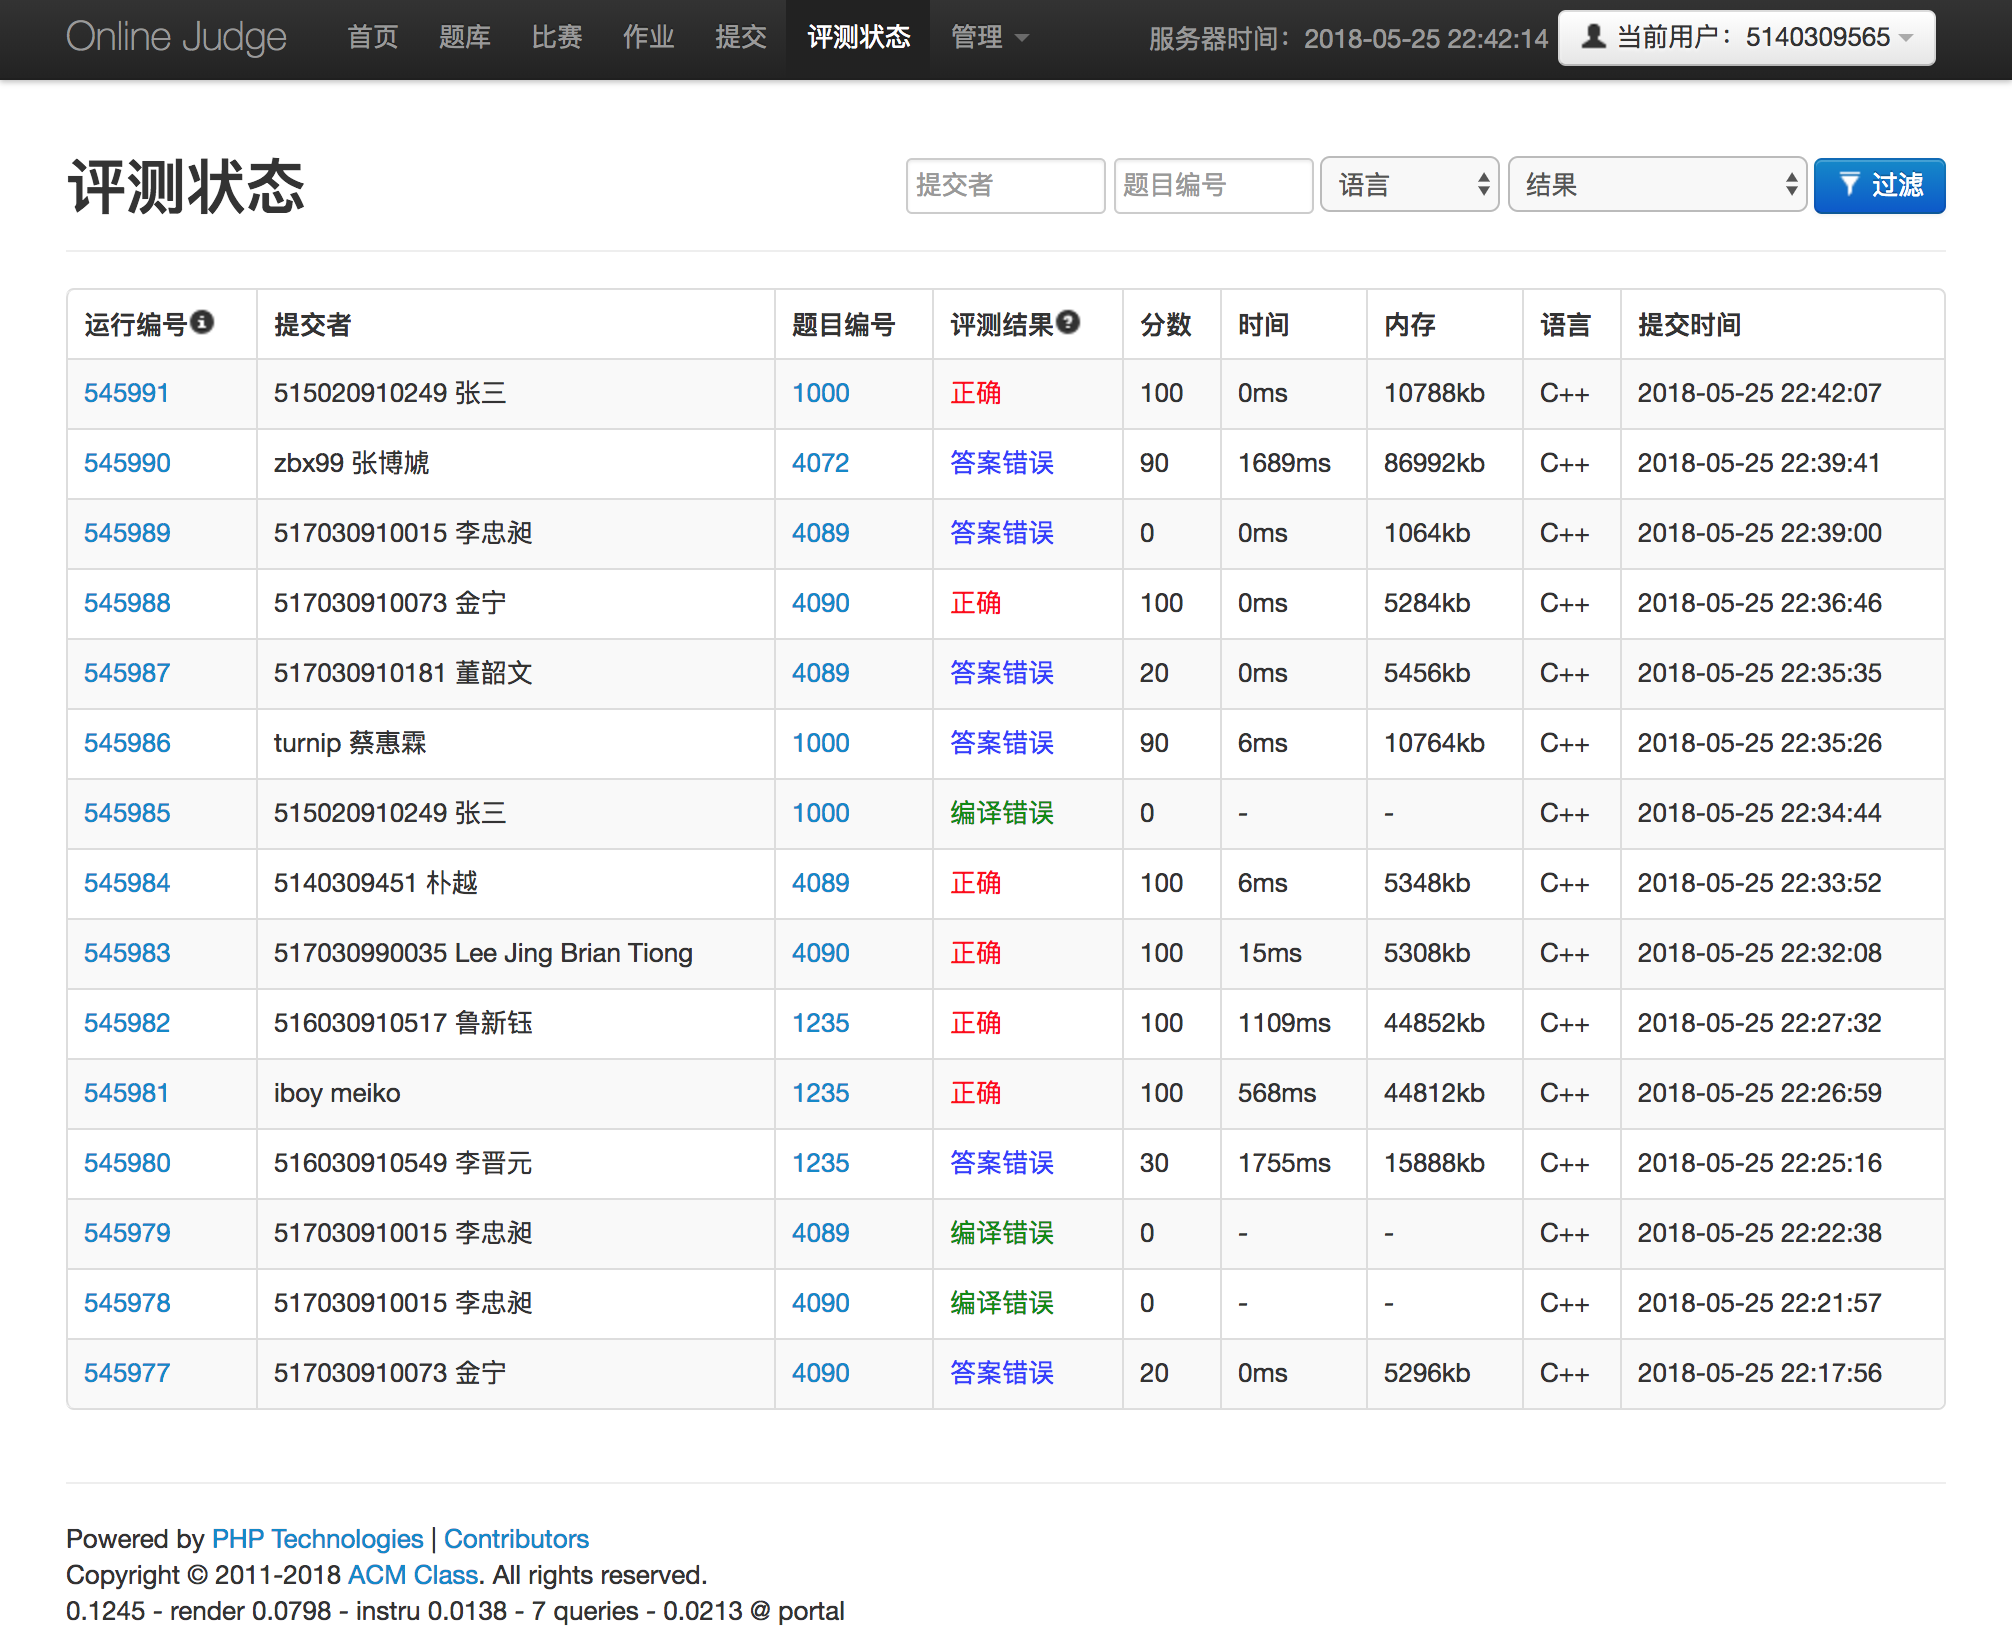
\includegraphics[width=0.62\textwidth]{img/acmoj.png}
        \caption{Snapshot of the status page of the OnlineJudge}
        \label{fig:acmoj}
    \end{figure}

    As ACM Honors Class expanded its influences, the Online Judge started to serve more people.
    Several departments, including School of Electronic Information and Electrical Engineering,
    School of Software, and IEEE Honors Class, use the Online Judge in programming related courses
    like Object-Oriented Programming.
    As for the Spring 2018 semester, the weekly submission on the Online Judge are more than ten thousand.

    Thanks to the Online Judge, our project has enough data to conduct experiments.

    \begin{itemize}
        \item The data we acquired span from October 1, 2011 to March 22, 2018.
        \item There are 7918 distinct users in total.
        \item There are 691 problems in total.
        \item There are 524,586 submissions in total, among which 507,269 is in the C++ language.
            We decided to only use submissions in C++ language.
            The number of correct C++ submissions is 158,684.
            Therefore, the ratio between accepted submissions and incorrect submissions is about $1:2$.
        \item Each submission contains following information:
            the user who submitted the solution,
            the problem identifier,
            the source code,
            the source code language
            the submission date and time,
            messages from the automatic grader,
            the verdict the automatic grader gave.
    \end{itemize}

\section{Data Preprocessing}

    Everyone deserves privacy. We do not want to leak users' information.
    For research purpose, it does not matter which person in real world an account corresponds to,
    as long as it is still distinguishable between different users.
    Therefore, we map the usernames in the submission records to unique numbers.

    \todo{looks too short}

\section{\texttt{dev-helper}: The Development Tool}

    During the early stage of development,
    it was helpful to check individual piece of data for varies of reasons,
    for example, it would be easy to spot some numeric values which do not make sense
    because of some trivial bugs during the feature extraction process.
    Also, randomly browsing the data might also help researchers to sense distribution of the data
    in some high-level semantics.

    Examining data in database management systems would be painful.
    Hence, we built a development tool called \texttt{dev-helper}
    that helps researchers better understand the data.
    \texttt{dev-helper} is a web application based on the \texttt{Flask}\cite{flask} web framework.
    It retrieve the raw data from the database and also read processed feature from the filesystem.
    It can show information of a specific problem to researchers.
    It also provides a function that displays a random problem.
    The information page of a problem includes the following parts (See Figure \ref{fig:dev-helper}):

    \begin{figure}[htp]
        \centering
        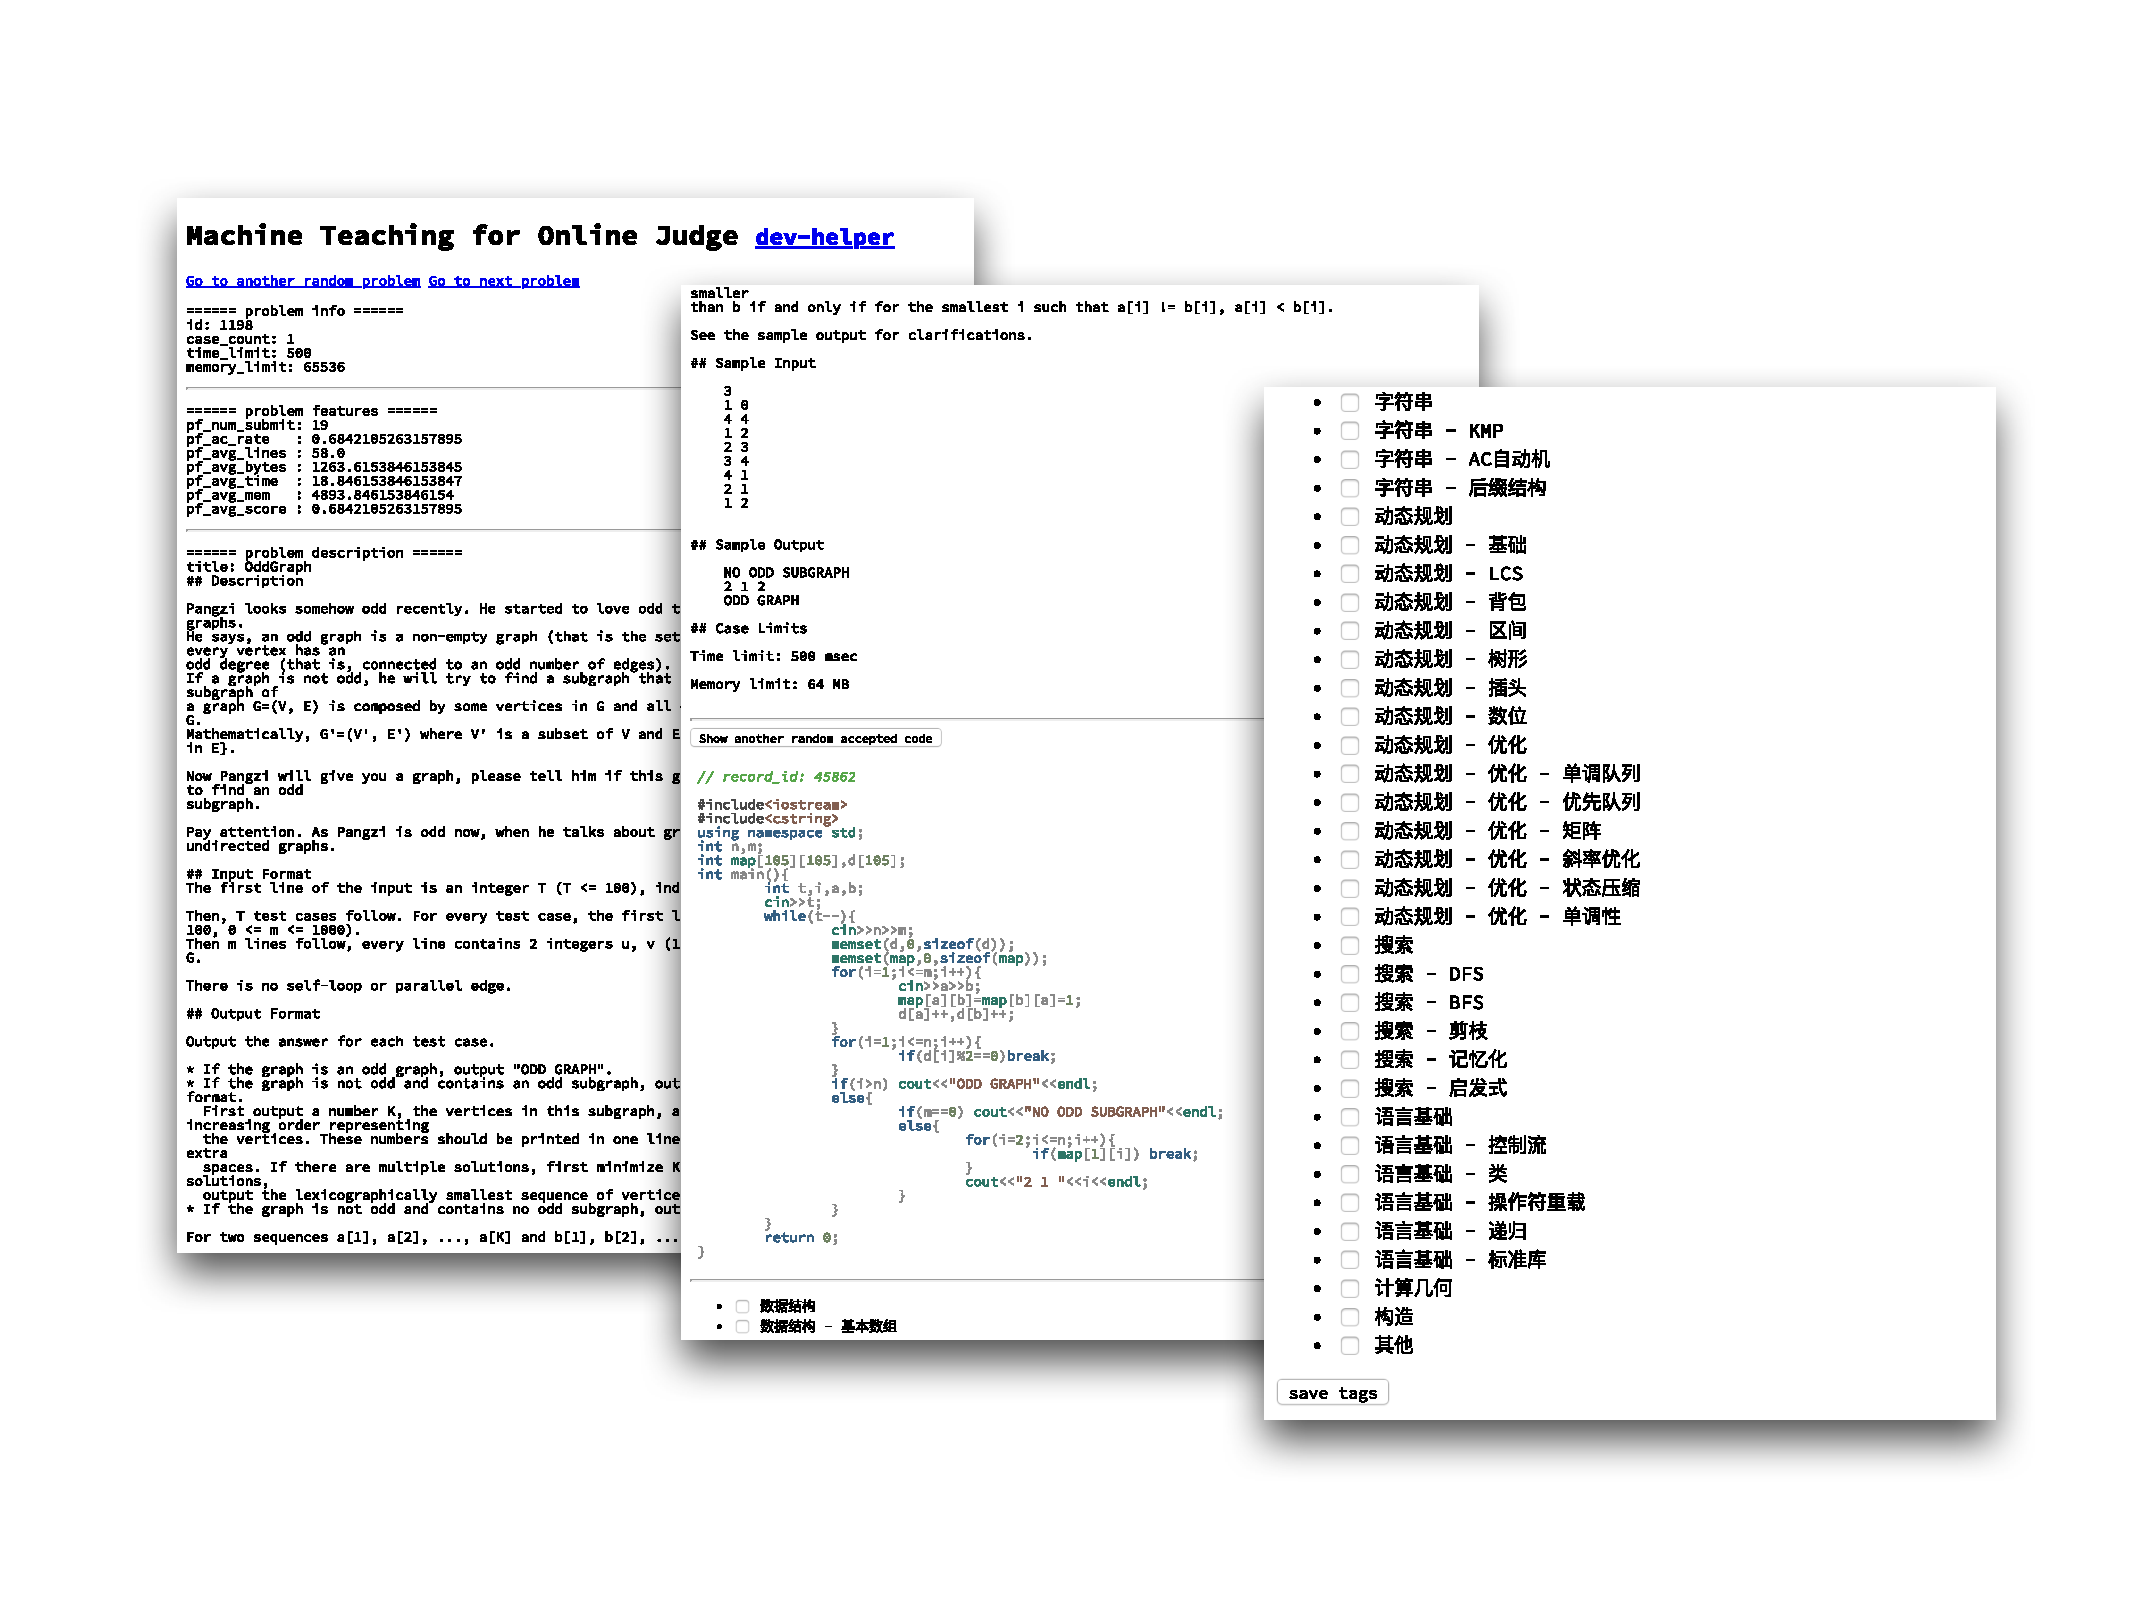
\includegraphics[width=0.62\textwidth]{img/dev-helper.pdf}
        \caption{Snapshot of \texttt{dev-helper}}
        \label{fig:dev-helper}
    \end{figure}

    \begin{itemize}
        \item The description of the problem.
        \item The metadata of the problem, including the problem identifier, time limit, memory limit, and so on.
        \item Values of the problem features.
        \item A random piece of accepted solution.
            There is also a button which when clicked will display another accepted solution randomly.
    \end{itemize}

    During the early development of this project, we found that \texttt{dev-helper} is indeed very helpful.

\section{Problem Tags}

    We categorize problems by its knowledge component, i.e., what types of knowledge this problem examines,
    such as dynamic programming, object-oriented programming, and so on.
    Tags are important features of a problem,
    but one flaw of our data is that it does not contain the tag information of problems.
    Therefore, we have to manually label the problems with a list of tags.

    In order to prevent different distributions of tags, we hired only one domain expert to label the problems.
    The domain expert has more than six years of experience in programming and competitive programming competitions,
    hence is surly capable of labeling the problems.
    We added a column of 87 problem tags on the problem information page on \texttt{dev-helper}.
    The experts read the description of a problem and several accepted solutions,
    then marked the corresponding tags, and finally clicked save.

    We believe that problem tags are important parts of the metadata of a problem.
    Notice that, although we manually tagged the problems afterwards and the domain expert is terrific,
    the one who knows the intention of a problem is its author.
    Therefore, we suggest that online judges ask problem authors submit problem tags along with the problems.
    Another alternative solution would be allowing users who have already solved the problem to tag the problem.
    One advantage of this method would be that users might discover alternative solutions to the problem
    which the problem author did not expect.

\section{Caveats on the Data Distribution}

    We found some interesting properties of the data from the Online Judge:

    Some problems added in contests or homework rarely have people attempting them
    after the period of the contest or the homework finished.
    In other words, those problems only served once, for a small group of the Online Judge.
    Hence, those problems might have difficulty comparing features like difficulty to other problems,
    due to the insufficient size and the high bias of the data.

    On the user side, similar bias exists.
    Users seldom if ever try to solve problems that is far above or below their levels.
    For example, a experienced OI participant would not pick a entry-level programming problem.
    Conversely, a student who begins to learn programming would not
    attempt to solve an advanced data structure problem.

    Although the Online Judge has users from all over the country,
    the majority usage of the Online Judge is still programming-related courses at SJTU.
    And few students do extra exercises on the Online Judge besides assignments which courses required .

    Consequently, the data distribution might be highly biased and clustered.

\section{Feature Extraction}

    \todo{make it longer: reason about the features; implementation details: concatenation}

    \subsection{Problem Features}

        We went through all submission records and extracted the problem features shown in Table \ref{table:problem features}.

        \begin{table}[hpbt]
        \begin{adjustwidth}{-1.5cm}{-1.5cm}
        \centering
        \begin{tabular}{lcp{12.5cm}}
            \hline
            Feature Name & Size & Description \\
            \hline
            {\footnotesize\verb|pf_tags|} & 87 &
                A multi-hot vector.\newline
                A component is 1 if the problem has the corresponding tag, otherwise 0. \\
            {\footnotesize\verb|pf_num_submit|} & 1 &
                The number of submissions to the problem. \\
            {\footnotesize\verb|pf_ac_rate|} & 1 &
                The ratio of the number of accepted solution to the total number of submissions. \\
            {\footnotesize\verb|pf_avg_lines|} & 1 &
                The average lines of source code of accepted solutions submitted to the problem. \\
            {\footnotesize\verb|pf_avg_bytes|} & 1 &
                The average bytes of source code of accepted solutions submitted to the problem. \\
            {\footnotesize\verb|pf_avg_time|} & 1 &
                The average total run time of accepted solutions submitted to the problem. \\
            {\footnotesize\verb|pf_avg_mem|} & 1 &
                The average maximum memory usage of accepted solutions submitted to the problem. \\
            {\footnotesize\verb|pf_avg_score|} & 1 &
                The average score of solutions submitted to the problem. \\
            \hline
        \end{tabular}
        \caption{Problem Features}
        \label{table:problem features}
        \end{adjustwidth}
        \end{table}

    \subsection{User Features and Context Features}

        For each submission record, we extracted the following user features shown in Table \ref{table:user features}.
        All of these features refers the user to the one who made the submission.
        All statistics count before the submission.
        Features above the separator is the basic feature set.
        The extended feature set includes all features in the table.

        \begin{table}[hpbt]
        % \begin{adjustwidth}{-1.5cm}{-1.5cm}
        \centering
        \begin{tabular}{lcp{10cm}}
            \hline
            Feature Name & Size & Description \\
            \hline
            {\footnotesize\verb|uf_num_submit|} & 1 &
                The number of total submissions made by this user before this submission. \\
            {\footnotesize\verb|uf_ac_rate|} & 1 &
                The ratio of accepted solutions to the total number of submissions. \\
            {\footnotesize\verb|uf_tag_num_submit|} & 87 &
                The number of total submissions grouped by problem tags. \\
            {\footnotesize\verb|uf_tag_ac_rate|} & 87 &
                The ratio of accepted solutions to the total number of submissions grouped by problem tags. \\
            \hline
            {\footnotesize\verb|uf_num_ac_problem|} & 1 &
                The number of solved problems. \\
            {\footnotesize\verb|uf_tag_num_ac_problem|} & 87 &
                The number of solved problems grouped by problem tags. \\
            {\footnotesize\verb|uf_num_one_ac|} & 1 &
                The number of problems that were solved by the first attempt to the problem. \\
            {\footnotesize\verb|uf_one_ac_rate|} & 1 &
                The ratio of the number of problems that were solved by the first attempt to the problem
                to the total number of solved problems. \\
            {\footnotesize\verb|uf_tag_num_one_ac|} & 87 &
                The number of problems that were solved by the first attempt to the problem grouped by problem tags. \\
            {\footnotesize\verb|uf_tag_one_ac_rate|} & 87 &
                The ratio of the number of problems that were solved by the first attempt to the problem
                to the total number of solved problems grouped by problem tags. \\
            {\footnotesize\verb|uf_avg_lines|} & 1 &
                The average lines of source code of submissions made by this user. \\
            {\footnotesize\verb|uf_tag_avg_lines|} & 87 &
                The average lines of source code of submissions made by this user grouped by problem tags.\\
            {\footnotesize\verb|uf_avg_bytes|} & 1 &
                The average bytes of source code of submissions made by this user. \\
            {\footnotesize\verb|uf_tag_avg_bytes|} & 87 &
                The average bytes of source code of submissions made by this user grouped by problem tags. \\
            {\footnotesize\verb|uf_avg_score|} & 1 &
                The average score of submissions made by this user. \\
            {\footnotesize\verb|uf_tag_avg_score|} & 87 &
                The average score of submissions made by this user grouped by problem tags. \\
            {\footnotesize\verb|uf_avg_submit_interval|} & 1 &
                The average time interval between consecutive submissions. \\
            {\footnotesize\verb|uf_tag_avg_submit_interval|} & 87 &
                The average time interval between consecutive submissions grouped by problem tags. \\
            {\footnotesize\verb|mf_is_first_attempt|} & 1 &
                Whether this user has attempted to do this problem before or not. \\
            {\footnotesize\verb|mf_has_ac|} & 1 &
                Whether this user has solved this problem before or not. \\
            {\footnotesize\verb|mf_num_attempt|} & 1 &
                The number of attempts this user has tried to do this problem before. \\
            {\footnotesize\verb|mf_avg_submit_interval|} & 1 &
                The average time interval between consecutive submissions to this problem. \\
            \hline
        \end{tabular}
        \caption[User Features]{\textbf{User Features}
            All of these features refers the user to the one who made the submission.
            All statistics count before the submission.
            Features above the separator is the basic feature set.
            The extended feature set includes all features in the table. }
        \label{table:user features}
        % \end{adjustwidth}
        \end{table}

        \todo{extended feature set}








